\newpage
\section{Suggested solutions: Discrete Fourier Transform}

\begin{enumerate}
\item Let $x[n]$ be a discrete-time signal of length $N$.

\begin{enumerate}[a)]
\item The spectral components in the DFT is given as $\omega_{k}=\frac{2\pi k}{NT_{s}}$. In units of hertz one has:
$$f_{k}=\frac{\omega_k}{2\pi}=\frac{k}{NT_{s}}=\frac{kf_{s}}{N}.$$

\item The DFT yields evenly spaces points in frequency domain corresponding to normalized angular frequencies of:
$$\hat{\omega}_{k}=\frac{2\pi k}{N}.$$
In other words, the resolution is:
$$\Delta\hat{\omega}=\frac{2\pi (k+1)}{N}-\frac{2\pi k}{N}=\frac{2\pi}{N}.$$
In units of hertz, we get:
$$\Delta f = \frac{\Delta\omega_{k}}{2\pi}=\frac{\Delta\hat{\omega}}{2\pi T_{s}}=\frac{2\pi}{N}\frac{1}{2\pi T_{s}}=\frac{1}{N T_{s}}=\frac{f_{s}}{N}.$$
Having used that $\hat{\omega}=\omega_{k}T_{s}$. If we want to have a resolution of $\Delta f=0.1$ Hz, then we must choose $N$, so that:
$$N=\frac{f_{s}}{\Delta f}=\frac{17\cdot 10^{3}\ \text{Hz}}{0.1\ \text{Hz}}=\underline{\underline{170000}}.$$
\end{enumerate}

\item Let $x[n]$ be a discrete-time signal of the form:
$$x[n]=\cos(\hat{\omega}_0 n)+2\cos(\hat{\omega}_1 n)+3\cos(\hat{\omega}_2 n).$$

\begin{enumerate}[a)]
\item Have that $\hat{\omega}=\omega T_{s}$, where $\omega$ is in units of radians per second and $\hat{\omega}$ is in units of radians per sample. Furthermore, have that $\omega=2\pi f$, where $f$ is in units of hertz, so that $\hat{\omega}=2\pi f T_{s}$. In other words:
\begin{align*}
    f_{0} &= \frac{\hat{\omega}_{0}}{2\pi T_{s}}=\frac{2\pi (4000)T_{s}}{2\pi T_{s}}=\underline{\underline{4000\ \text{Hz}}},  \\
    f_{1} &= \frac{\hat{\omega}_{1}}{2\pi T_{s}}=\frac{2\pi (1000)T_{s}}{2\pi T_{s}}=\underline{\underline{1000\ \text{Hz}}},  \\
    f_{2} &= \frac{T_{s}}{2\pi T_{s}}=\frac{2\pi (2500)T_{s}}{2\pi T_{s}}=\underline{\underline{2500\  \text{Hz}}}, 
\end{align*}
where the values obtained for the normalized frequency is read from the Python code. 

\item Let $x[n]$ be as above, then the signal is periodic if: for all $\hat{\omega}_{i},\hat{\omega}_{j}$ one has $\hat{\omega}_{i}/\hat{\omega}_{j}\in\mathbb{Q}$. This is the case here, as:
\begin{align*}
    \hat{\omega}_{0}/\hat{\omega}_{1} &= 4,\\ 
    \hat{\omega}_{1}/\hat{\omega}_{2} &= 2/5,\\
    \hat{\omega}_{2}/\hat{\omega}_{0} &= 8/5,
\end{align*}
for which all are rational numbers, hence $x[n]$ is periodic. 
We've only checked some choices of indices, as the reciprocal of a rational number is also a rational number. 

To compute the period of the signal, use the fact that the fundamental period is related to the greatest common divisor (GCD) of the angular frequencies. To compute the GCD of three terms, one can use the fact that: $\hat{\omega}=\gcd(\hat{\omega}_{0},\hat{\omega}_{1},\hat{\omega}_{2})=\gcd(\hat{\omega}_{0},\gcd(\hat{\omega}_{1},\hat{\omega}_{2}))$. You can compute the $\gcd$ in Python if you ignore the $2\pi T_{s}$ part, using the \verb|math| module with the function \verb|gcd|. Doing this gives $\hat{\omega}=2\pi500T_{s}$ in units of radians per sample. To obtain the period in units of samples:
$$N=\frac{2\pi}{\hat{\omega}}=\frac{2\pi}{2\pi500T_{s}}=20 \ \text{samples}.$$
The period in units of seconds, is then:
$$T=\frac{2\pi}{\omega}=\frac{2\pi T_{s}}{\hat{\omega}}=\frac{2\pi T_{s}}{2\pi500T_{s}}=\frac{1}{500}=0.002 \ \text{s},$$
as $\hat{\omega}=\omega T_{s}$, so the signal is periodic with a period of 20 samples, or 0.0002 seconds. 

\item Listing \ref{code:ex152c} shows a way to obtain units of hertz on the x-axis. The output of Listing \ref{code:ex152c} is shown in Figure \ref{fig:ex15_c.png}. 
\lstinputlisting[language=Python,caption=Plot with units of hertz on the x-axis,label=code:ex152c,linerange={1-21}]{ch15/code/ex15_2c.py}

\begin{marginfigure}
    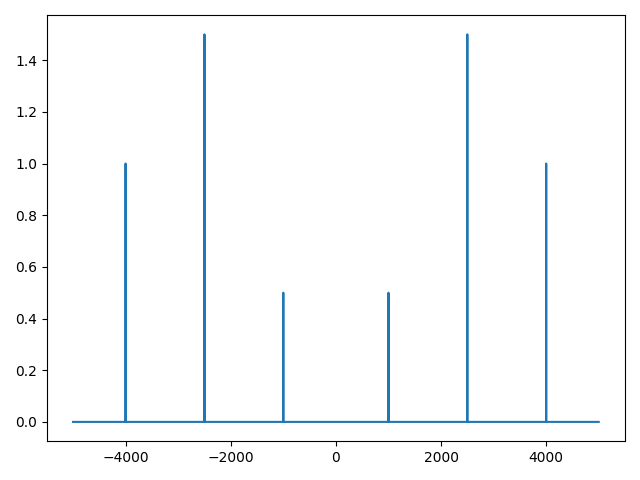
\includegraphics[width=7.0cm,height=6.8cm]{ch15/figures/ex15_c.png}
    \caption{The magnitudes of six spectral components, but units of hertz on the x-axis}
    \label{fig:ex15_c.png}
    \end{marginfigure}

\end{enumerate}

\end{enumerate}
